\documentclass[12pt,journal,compsoc]{IEEEtran}

\usepackage{amsmath}
\usepackage{graphicx}

\begin{document}

\title{Data transfer, Control Systems, and Sensors\\
	CMPE 185 Final Project}
\author{Maxwell~Bradley, Kodiak~North, and Zane~Bradley}

\date{\today} % leaving the brackets empty omits the date
% To input the current date, you can type: \date{\today}

% The paper headers
\markboth{Data transfer, Control Systems, and Sensors}%
{Bradley, M; North, K; Bradley, Z\MakeLowercase{\textit{et al.}}: CMPE185}

\IEEEcompsoctitleabstractindextext{%
\begin{abstract}
The purpose of this document is to teach someone the basics of EDIT THIS BRO. Readers will be able to insert tables, figures, mathematical formulas, bibliographies, and references by the end of the tutorial.
\end{abstract}

\begin{IEEEkeywords}
Aircraft, Airplane, RC Airplane, UAV, Autonomous, Wildfire, Wildfire Detection, Search and Rescue
\end{IEEEkeywords}}

\maketitle

\tableofcontents 

\section{Project Introduction}

\IEEEPARstart{F}{orever} Flight is a persistent aerial monitoring system to detect wildfires in fire-prone areas. It will consist of a plane with a mounted IR camera to detect fires below and a flight controller capable of autopilot, guidable with GPS waypoints sent from a laptop computer on the ground. This project was named ‘Forever Flight' for its goal of never having to recharge its batteries, staying aloft and performing fire detection while the sun is up, charging back up from solar energy and our power regenerative mechanisms. 

This project was inspired by the recent California wildfires like the Camp Fire, a 2018 fire in Northern California that caused \$16.5 billion in damage and claimed 86 lives [1]. The reason that these fires were so deadly is because there was no early warning system that detected the fire before it started ripping through towns like Paradise, California. The team hopes that Forever Flight will prevent fires like this.

% MAX B
\section{Data Transfer}
\subsection{Introduction}
An important part of this project is the data transfer from the plane to the ground station. This transfer contains a huge amount of different kinds of data, such as fire detection stats, fire detection processing, GPS coordinates, and more. Getting this kind of information out of the plane can be challenging because of the flight controller's running overhead and varying transmission protocol versions. This section of the paper will talk about the communication of data between the in-flight aircraft and the ground control station read by our product user.

\subsection{Materials and Material Background}
A multitude of different components make up the data transmission path between the plane itself and the ground station. Each of those parts will now be discussed in detail.
\subsubsection{Pixhawk Flight Controller}
The Pixhawk flight controller is the main brain of the entire plane. It receives IR information from the IR sensor mounted downwards pointing at the ground through a serial communication port (using the I2C protocol). The Pixhawk is where the majority of the data transfer work occurs in the second version of the data transmission design. It uses an overall system scheduler to decide when to send MAVLink packets to the ground station. Within the function that is scheduled in the overall scheduler, a smaller MAVLink scheduler exists. Within the MAVLink scheduler, one of a large group of packets is selected and sent over whatever telemetry port MAVLink is configured to use.
\subsubsection{MAVLink}
MAVLink is a protocol commonly used between drones and ground stations. Most autopilots use MAVLink to both send and receive packets to and from the ground station, respectively. Its packet structure is described in the following picture.
% MAX PICTURE 1
\begin{figure}[h!]
\hspace*{0cm}
\centering
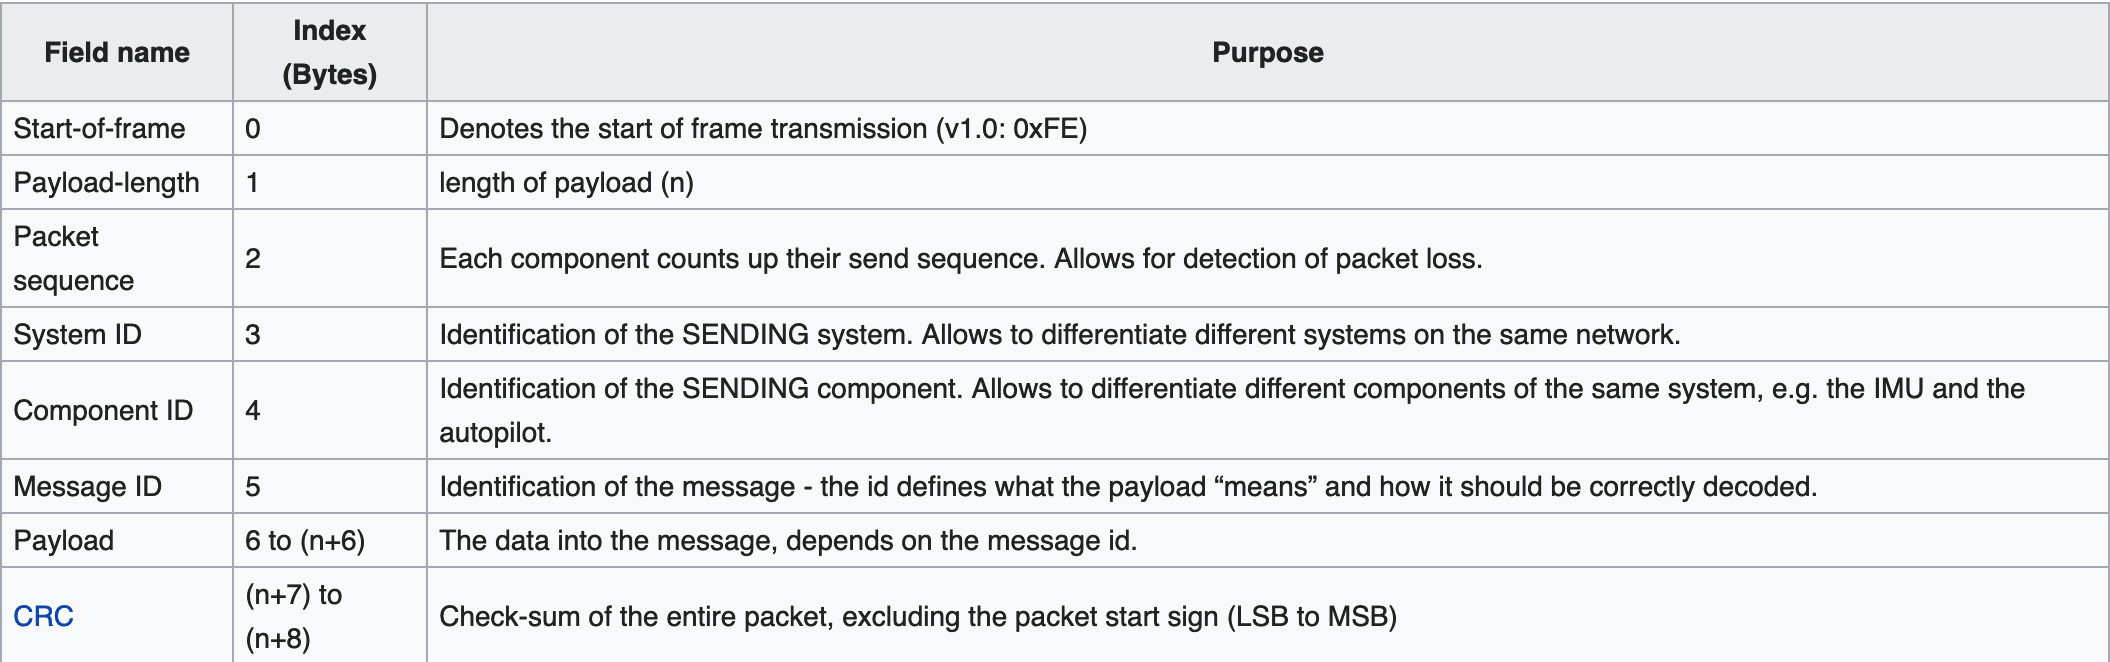
\includegraphics[width=3in]{MavlinkStructure.png}
\caption{Max B1}
\label{mavStruct}
\end{figure}

The start frame transmission is the hex character set 0xFE, which tells the ground station that the packet is incoming. The next byte tells the receiver how many bytes in the payload to expect. The next set of bytes are for identifying the system sending the message, the component sending the message, and the packet sequence.

The most important part of this packet is the message id, the 5th byte in the index. This byte signals which MAVLink message the incoming data corresponds to. MAVLink messages are defined in a file called common.xml. Every message coming in indexes to one of the messages in the common.xml file. For instance, several times a second a ‘heartbeat' message is sent from the plane to the ground station. This message is declared in the common.xml file as having ID 0. When the ground station receives this message, it reads that xml file, looking for a message definition that matches the incoming ID. When it finds it, it interprets the payload attached to the MAVLink message as the attributes associated with the message definition in the xml file. 
The autopilot that was chosen for this project uses the MAVLink protocol to communicate with the ground station. As a result, the team has become very familiar with its function. 
\subsubsection{ArduPilot}
After looking at all the free and open source autopilots out there on the market, Ardupilot, an open source autopilot that runs on the Pixhawk4, was selected. This firmware can be run on a variety of different platforms: there is an ArduSub, an ArduCopter, an ArduTractor, and obviously an ArduPlane. The flight controller for this project uses the ArduPlane version. 

This autopilot is written in C++, and has a relatively small code base for the ArduPlane itself. It's most important parts consist of a main plane scheduler, a MAVLink sending module, and a huge header file that includes all the important modules from the libraries and from the plane folder itself. 

The majority of the meat for the ArduPlane module is contained in the libraries. The programmers for ArduPilot wisely chose to combine the largesse of the code in libraries which all different vehicle versions that run ArduPilot (ArduPlane, ArduSub, ArduTractor, etc.) use. These libraries contain code for sending MAVLink that can be used between vehicles, hardware abstraction layers, control systems, and plenty more. 
\subsubsection{Telemetry Module}
The team landed on using the 3DR Radio Telemetry Kit. This set of transmitters and receivers use the frequency 916MHz. The flight controller uses this link to send flight data. The ground station sends GPS coordinates for the plane to track to on over this link as well. A picture of this module is below.
% MAX PICTURE 2
\begin{figure}[h!]
\hspace*{0cm}
\centering
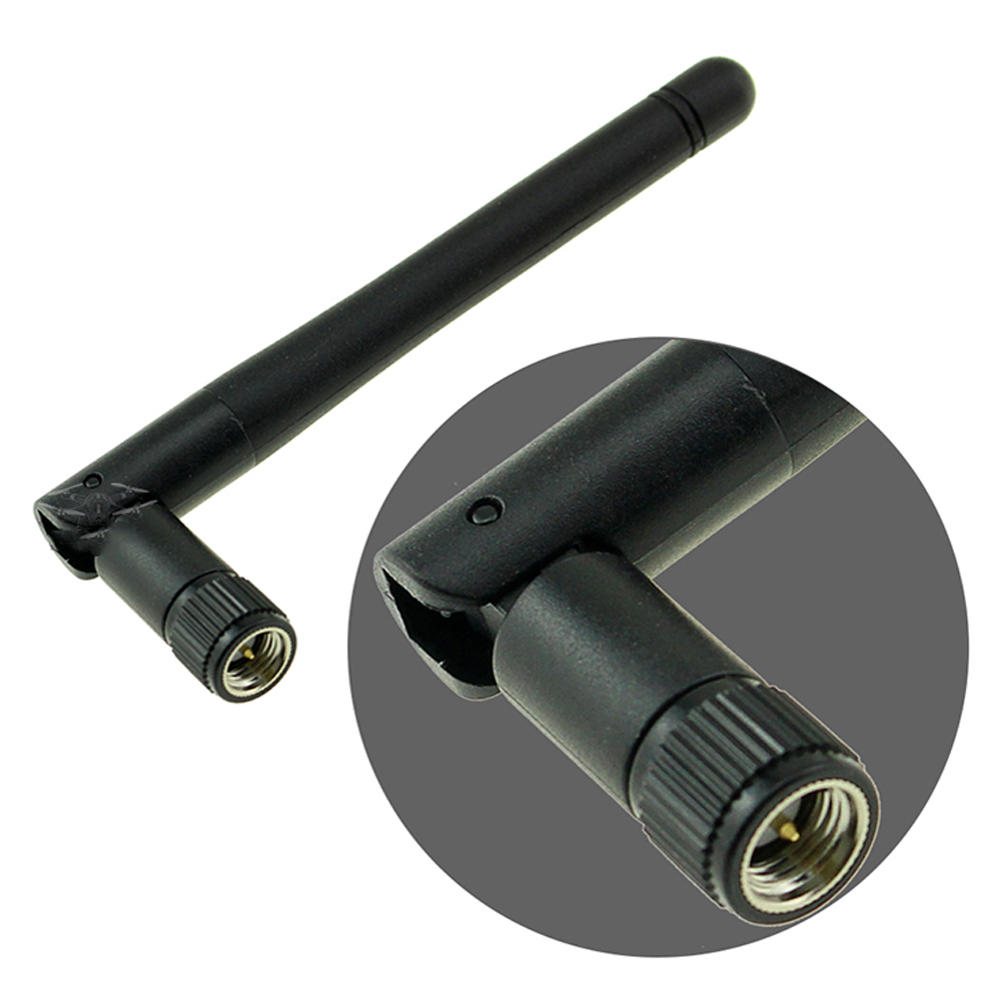
\includegraphics[scale=.125]{telemmodule.jpg}
\caption{Max B1}
\label{mavStruct}
\end{figure}

\section{Results and Discussion}
This section of the paper will be about the overall set up of the system, the design process, and the problems that were encountered on the way.
\subsubsection{System Set Up}
Our data transmission system starts in the Pixhawk scheduler code in the main file called ArduPlane.cpp. The flight controller is essentially a microcontroller without an operating system, which means that it needs to implement a scheduling system that figures out which process of the hundreds of processes competing for the processor to run. This is what the scheduler looks like in code:
% MAX PICTURE 3
\begin{figure}[h!]
\hspace*{0cm}
\centering
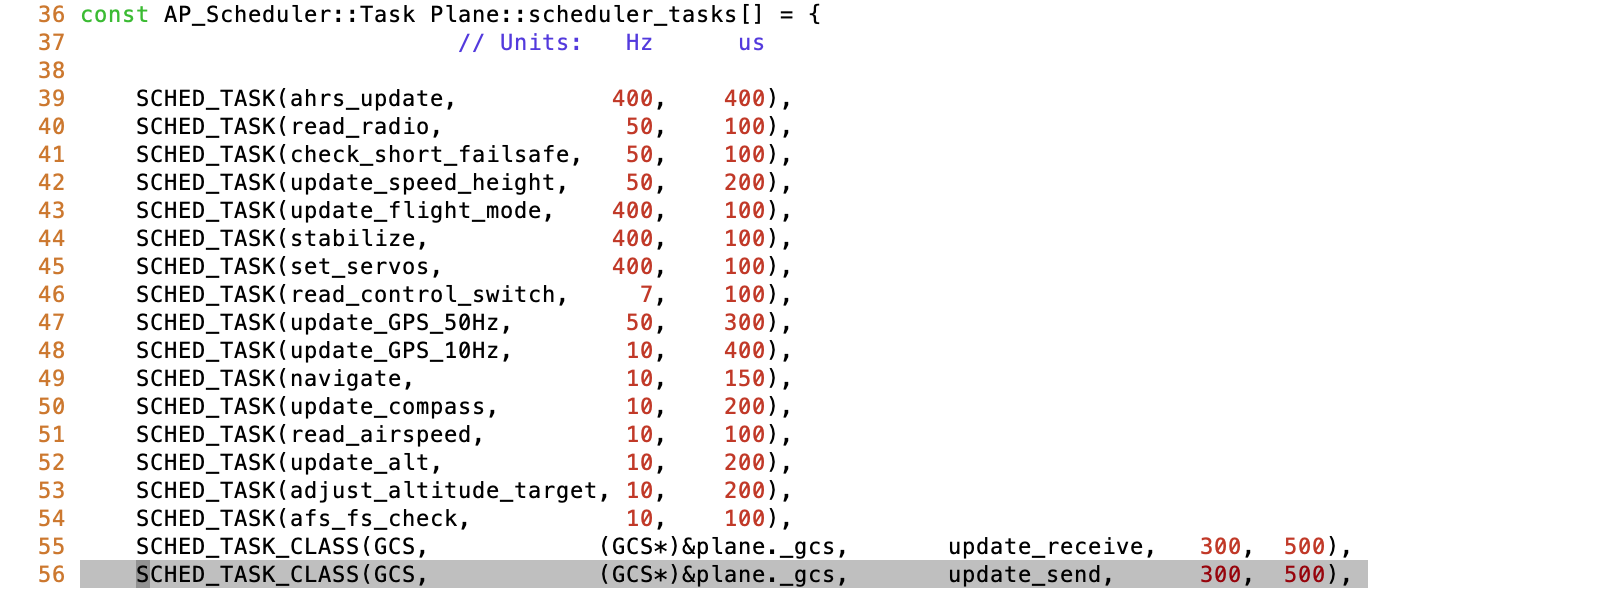
\includegraphics[width=3in]{Scheduler.png}
\caption{Max B3}
\label{mavSched}
\end{figure}

The highlighted line of code schedules the GCS sending module, which calls functions to use the MAVLink link between the ground station and the plane. Diving deeper into the code base in the plane folder, there is the GCS\_MAVLink.cpp file that contains the functions to actually go about sending the message. This is where changes started:
% MAX PICTURE 4
\begin{figure}[h!]
\hspace*{0cm}
\centering
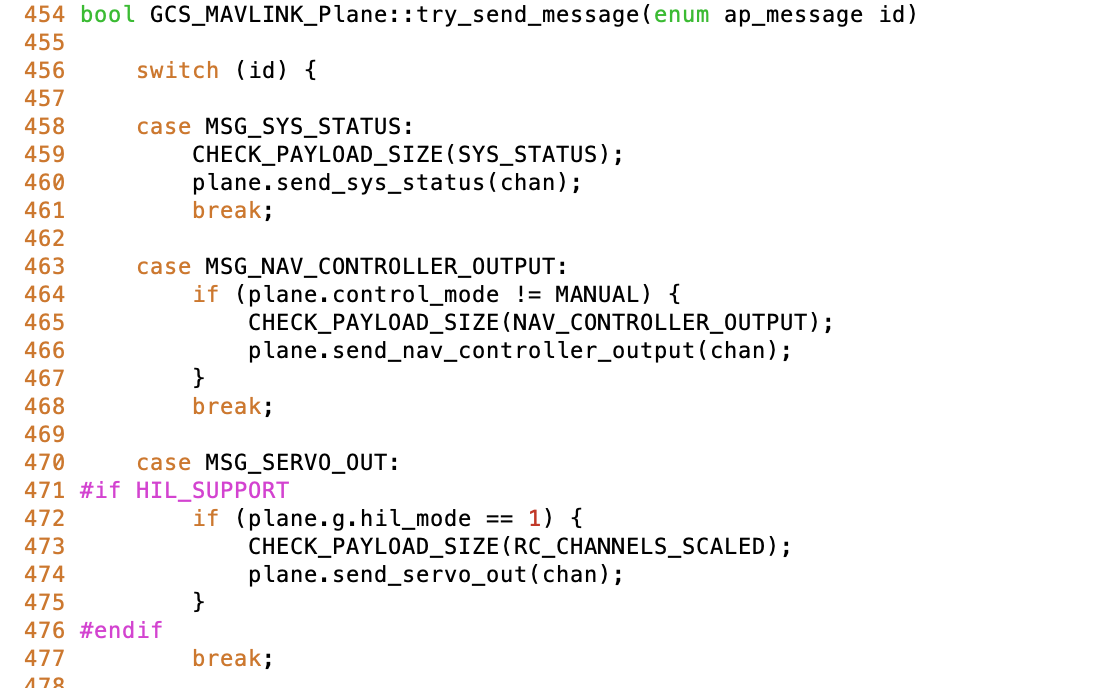
\includegraphics[width=3in]{GCS_Mavlink.png}
\caption{Max B4}
\label{gcsMav}
\end{figure}

As a backup to the above function, ArduPilot also implemented a function that all vehicles under the ArduPilot umbrella use. If none of the IDs passed into the try\_send\_message function matched, it would fall into the try\_send\_message that was defined in the libraries of ArduPilot.  This was good for overall project structuring, but made finding the actual implementation of MAVLink sending very challenging. 

Below is the fallback function at the end of the previous function that links the plane implementation to the common MAVLink packets that all ArduPilot vehicles use. This function is contained in the library files that all ArduPilot vehicles contain. 
% MAX PICTURE 5
\begin{figure}[h!]
\hspace*{0cm}
\centering
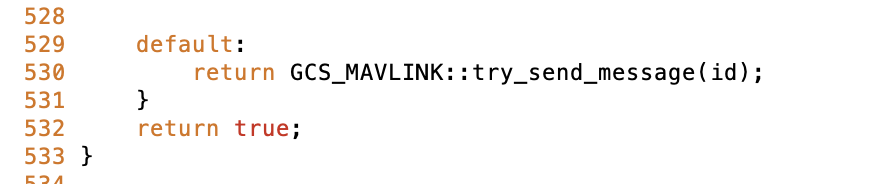
\includegraphics[width=3in]{Fallthrough.png}
\caption{Max B5}
\label{fallthrough}
\end{figure}

By editing code in either the library function or the ArduPlane specific function, it was possible to make changes to the MAVLink messages that were being sent to the ground station. 
Changes were made to existing MAVLink definitions rather than create new ones because of the difficulty in changing the MAVLink protocol version from version 1.0 to version 2.0 (please view the problems section for more information on this issue). To edit MAVLink message definitions, changes needed to be made in the common.xml or ardupilotmega.xml files.
\subsubsection{Design Process}
The design process was begun by trying to prevent the flight controller from having to handle any of the data transmission at all. Instead, the original plan was to have a Teensy microcontroller serve as the gateway between the ground station on the ground and the plane up in the sky. The first thing that was done was to set up a UART link between the Teensy and the flight controller, sending over information that would eventually be relayed to the ground station. The overall structure looked like this:
% MAX PICTURE 6
\begin{figure}[h!]
\hspace*{0cm}
\centering
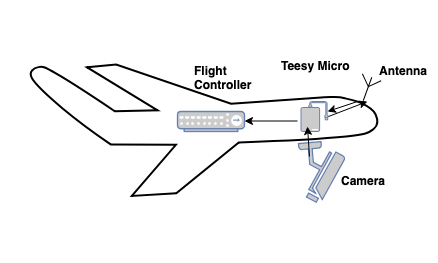
\includegraphics[width=3in]{Version1.png}
\caption{Max B6}
\label{version1}
\end{figure}

However, this set up became less than optimal when the incredible wealth of the already existing ground control software became apparent. It was discovered that the ground station software, Mission Planner, could be used to send GPS waypoints to the plane which it would then track to. The interface between the flight controller and the ground control station would only work if it could receive bytes from the ground station, and only allowing the Teensy access to the ground station would prevent this huge benefit from being realized. 
It didn't make sense to spend a lot of time designing a system where the Teensy read in fire detection data forwarded them to the flight controller. In addition, the small and underpowered Teesny with a processor clocked at 48 MHz could not hope to keep up with a flight controller clocked at over 3 times that. The Teensy was then removed from the picture, replaced with a more overloaded flight controller. A diagram of the current set up is below.
% MAX PICTURE 7
\begin{figure}[h!]
\hspace*{0cm}
\centering
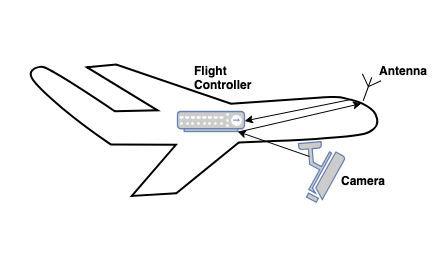
\includegraphics[width=3in]{Version2.png}
\caption{Max B7}
\label{version2}
\end{figure}

After the flight controller became the center of data processing and transmission, the design process began anew. The first important thing to do was to get a good understanding all of the underlying code for data transmission in the ArduPilot framework. After tracking down the control flow through the different files which eventually ended in in the library file that all ArduPilot vehicles used, the next step was to add a particular message to the common.xml file which contained the MAVLink message definitions. 

Due to a parameter problem that will be covered in-depth in the problems part of this discussion, it was necessary to overwrite one of the existing MAVLink definitions. The MAV\_CMD\_NAV\_LAND with ID 21 message was selected because the plane should never be allowed to land automatically This message was overwritten with a custom packet that contained fire detection data. This packet would only be sent when the sensing apparatus actually detected a fire, even though the message would be scheduled for sending at least once a second. The simple control flow of this setup is as follows.
% MAX PICTURE 8
\begin{figure}[h!]
\hspace*{0cm}
\centering
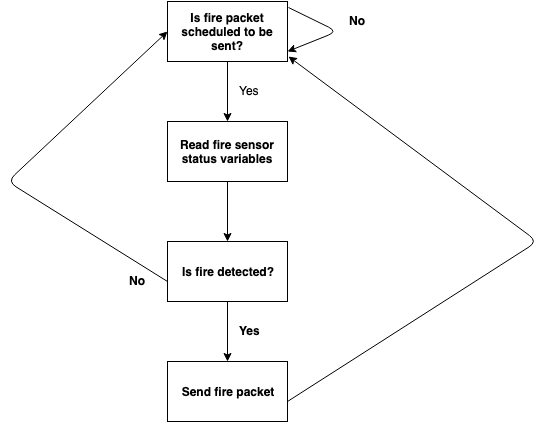
\includegraphics[width=3in]{Sending.png}
\caption{Max B8}
\label{sending}
\end{figure}

For the ground station that would receive messages, a Python script that used the Python package PyMavlink's submodule mavuti was used. This allowed a reading of the serial port and a parsing/translation of the incoming MAVLink message into human readable data. The associated data was then used to make plots, such as the following that plots latitude and longitude from the incoming GPS data packets.
% MAX PICTURE 9
\begin{figure}[h!]
\hspace*{0cm}
\centering
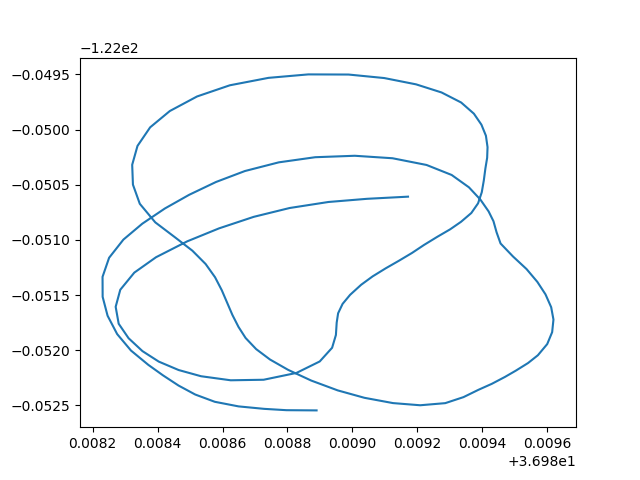
\includegraphics[width=3in]{flight02-22-2019_maiden.png}
\caption{Plot of the aircraft's maiden flight using GPS coordinates that were logged in real time via the telemetry link.}
\label{maidenFlightPlot}
\end{figure}

This allows for the collection of real time flight data which can be very different from the data read from a wind tunnel in the lab. 

\subsubsection{Design Problems}
The biggest and most enveloping design problem that was encountered during this project was changing the MAVLink protocol version. Please note the MAVLink byte structure referred to in the next few sentences is the first diagram of this section of the report. The 5th byte of the packet designates the ID number that corresponds to the MAVLink message. This limits the total number of incoming messages to 256. The common.xml file contains message definitions up to 256. Due to the limited number of bits (8) that correspond to the incoming ID, there are only 256 possible messages that can be sent. This is why overwriting the already defined messages in the common.xml file is needed. Creating new messages with an ID value greater than 255 would not be able to be sent by the current MAVLink protocol. Originally, a custom packet with an ID value of 11065 was created and the sending function for that specific packet was called. However, nothing was sent, not even garbage. This along with the packet header of 0xFE made it very clear that the first version of the MAVLink protocol was being used rather than the updated and more flexible MAVLink version 2. Overwriting the message was a necessary evil to send custom packets unfortunately. 

The changing of this protocol is badly documented on the ArduPilot website. Eventually, a manual change using the MAVProxy python library was attempted (specifically changing the protocol version parameter of the MAVLink version), but MAVLink 1 packets continued to be sent. In the interest of time, it was decided that simply overwriting the useless packets defined for MAVLink 1 was the best course of action.

\subsection{Data Transfer Conclusion}
Data transmission software is essential to pulling real time data that closely reflects and explains the events that occured during flight. Even though the open source autopilot is incredibly difficult to parse through and overall not very well written by industry computer science standards, it can be manipulated to add custom MAVLink functionality. 

An added problem of working with this flight controller is the time and processing constraints that adding a custom bit of functionality to an already extremely overtasked system come with. However, by keeping subroutines short, it was possible to add a good amount of data collecting and transmission software to an already built system.

% Kodiak
\section{Control System}
\subsection{Introduction}
The control systems section will explore the mysterious art of controlling planes without a pilot on-board. The overall plan is to control the aircraft in an optimal way to detect wildfires, but for now, we are just focused on control in general.

\subsubsection{Treating the Aircraft as a Dubins Vehicle}
All information in this section was found in \cite{S-U-A}, chapters 9 and 10. These chapters focus mainly on creating a model for guidance and path following. Using coordinate frame matrices to resemble flight, we can model aircraft dynamics along with outside forces with the following equation (eq 9.9 in \cite{S-U-A}):
\[ \begin{pmatrix}
\dot{p_n} \\
\dot{p_e} \\
\dot{h}
\end{pmatrix}  
= V_a \begin{pmatrix}
cos(\psi) \\
sin(\psi) \\
0
\end{pmatrix}
+ \begin{pmatrix}
w_n \\
w_e \\
0
\end{pmatrix}
\]
It essentially says that the angular roll rate $\dot{p}$, and the rate of change in altitude $\dot{h}$ are equivalent to the airspeed $V_a$ times the cosine and sine of the yaw angle $\psi$ plus the wind direction $w$. Note that aerodynamic forces acting on the aircraft body are removed from this equation to greatly simplify it. The equation assumes the aircraft maintains a steady altitude to model it like a dubins vehicle with a forward velocity and a turning rate. The airplane is then controlled by increasing or decreasing the veloticy and changing the turning rate. Below in Figure \ref{f8} is a plot of a dubins vehicle moving in a figure-eight pattern:
\begin{figure}[h!]
\hspace*{0cm}
\centering
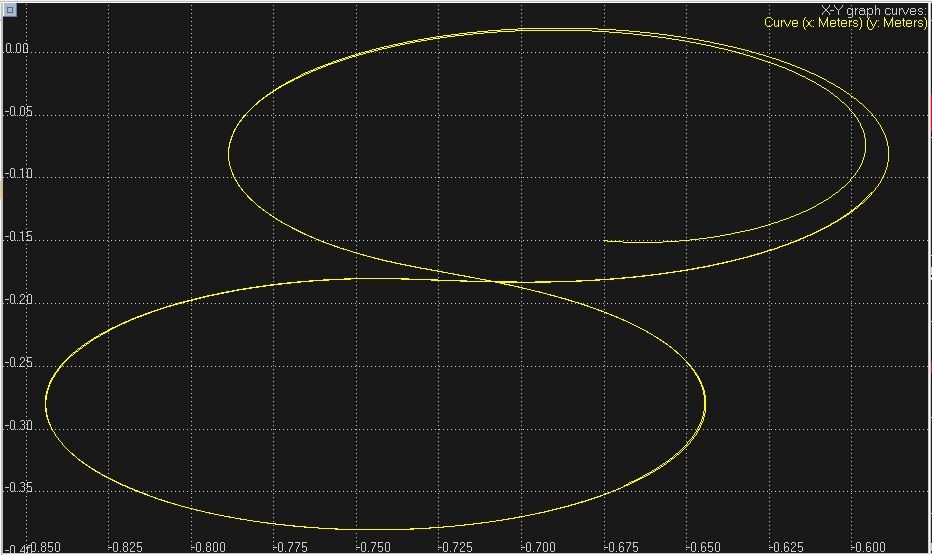
\includegraphics[width=3in]{dubins_fig8.jpg}
\caption{Dubins vehicle programmed to move in a figure-eight pattern by holding a constant velocity and changing the sign of its turning rate at a specific time interval. An airplane at a constant forward velocity and altitude can be modeled in a similar fashion. Note this picture was taken from a project the author completed for CMPE 141.}
\label{f8}
\end{figure}
This idea is particularly useful for Unmanned Aerial Vehicles (UAVs), which do not perform aerobatic maneuvers and usually maintain a steady altitude to scan an area. Engineers can basically pretend their UAV is a dubins vehicle once it reaches its cruising altitude! We can then relate the turning rate along the yaw axis $\dot{\psi}$ to gravity, velocity, and the roll angle $\phi$ with the following equation (eq 9.14 in \cite{S-U-A}):
\[ \dot{\psi} = \frac{g}{V_a}tan(\phi) \]
It is important because it gives us a direct relation from roll angle to yaw rate. This equation is similar to the steering wheel on a car - it is rolled left and right to make the car yaw left and right. In this case, the aircraft itself is the steering wheel rolling left and right to yaw back and forth. We now have everything we need to control a UAV like a dubins vehicle using the roll angle to modify turning rate, and the motor to adjust its speed.

\subsubsection{Aircraft Ground Control Stations}
All information in this section was found in \cite{U-A-D}, chapter 8. A ground control station is something that can apply the dubins vehicle model as the UAV is in the air. As an operator plans the flight, the ground control software will calculate the turning rate (i.e. roll angle) required to follow the path. If the turning rate is unachievable, the software must notify the operator, or perform longer, wider maneuvers to correct for the error and follow the path as close as possible. This is one of many reasons why ground station are important tools for a UAVs. Their other purposes are to allow an operator to track/plan the mission, observe flight status, and pilot the aircraft. ``Depending upon range and type of mission (complexity of the UAV system), smaller UAVs are controlled via visual contact (manual real-time control), while the larger ones are equipped with a communication system (engage stored on-board flight plans)" (Sadraey, page 141). Some UAVs are not fully autonomous, so an operator must fly it using a laptop with ground control software. UAVs also have various sensors on them like a weapon position sensor, altimeter, airspeed sensor, intertial measurement unit (IMU), and many more. If the ground control station operator notices anything is acting funny, he can take full control and act accordingly.
\begin{figure}[h!]
\hspace*{0cm}
\centering
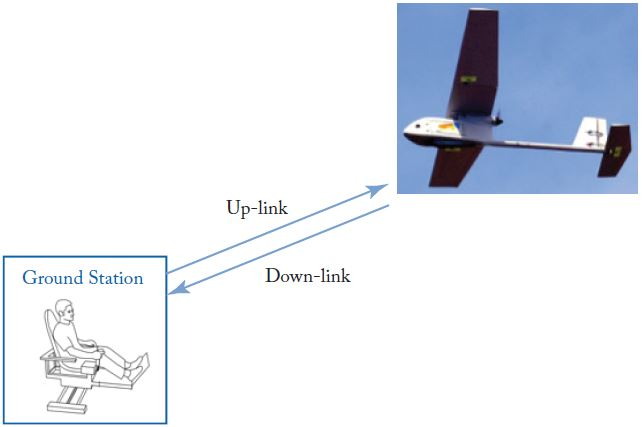
\includegraphics[width=3in]{groundControl.jpg}
\caption{Diagram displaying and operator of a ground control station to pilot an aircraft. Most stations do not require the operator to sit in a cockpit-like seat, but the exaggeration is useful for a novice UAV enthusiast. This image was found in \cite{U-A-D}, page 142, Figure 8.1.}
\label{gcDiagram}
\end{figure}
Normally, there are two operators to a ground control station; the vehicle flight operator and the mission payload operator. The flight operator is in charge of keeping the machine in the air, while the payload operator interfaces with other aircraft systems. This could be aiming and firing guns, taking weather data, or gathering recon information for teams on the ground. These operators play a crucial role because although the plane can fly mostly, or fully autonomously, ``most UAV losses are attributed to operator errors" (Sadraey, page 143). The operators must be comfortable when working with these expensive devices or else their state of mind will fatigue, and the chances of making a mistake increase. It is important to keep comfort in mind when desigining a ground control station.

\subsubsection{Glider Soaring via Reinforcement Learning in the Field}
All information in this section was found in \cite{GliderBirds}. One way to extend the flight time of a small, unmanned aircraft is to utilize thermals and updrafts similar to the way birds do. Physicists at UC San Diego figured out how to do exactly that by using reinforcement learning - a type of machine learning.
\begin{figure}[h!]
\hspace*{0cm}
\centering
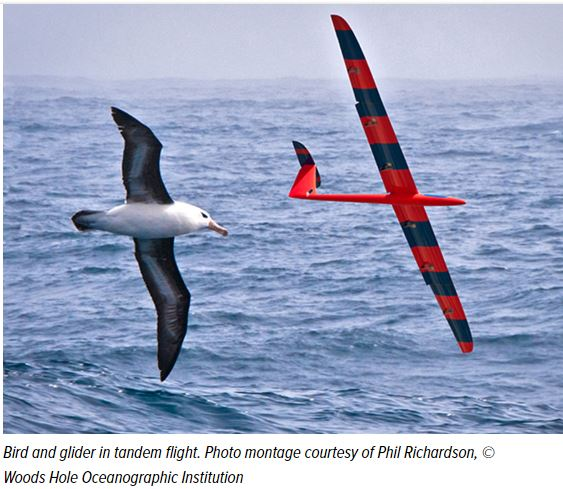
\includegraphics[width=3in]{gliderAndBird.jpg}
\caption{Here is one of the gliders used in the testing process flying in tandem with a seagull. The two both have the same attitude to achieve the most lift out of the thermal or updraft they are flying through. This image was found in \cite{gbArticle}.}
\label{gliderAndBird}
\end{figure}
Reinforcement learning is essentially a way for a system to learn based on trial and error; if it preforms an action and things go well, it remembers that as a good situation, while on the other hand, poor situations from bad maneuvers are kept in the ``don't do again" list. The physicists started by simulating gliders in turbulent wind flow to find important parameters that improve navigation through a thermal. They then moved on to testing a real plane with a 2 meter wingspan. The plane was equipped with a flight controller running modified ArduPlane code to pilot the aircraft through updrafts. Researchers soon discovered that they needed to write algorithms to estimate ``environmental cues" to maneuver the glider in such a way to gain the most lift out of the environment. For example, when a pocket of greater lift is at a diagonal to the aircraft's forward heading, banking in a proper manner will generate more lift. This project intends to apply these properties to the Forever Flight aircraft to achieve a longer flight time when searching for wildfires.

\subsection{Conclusion}
Controlling an aircraft autonomously is no easy task. There is a lot of math and research that goes into it. Thankfully, many educated enthusiasts have summed up the fundamentals to help novices learn and contribute to the latest technology. By now, some of the important aspects of aircraft control, aircraft design, and flight extension have been discussed to introduce beginners to the art of UAVs. THIS COULD USE SOME MORE ADDED

\section{Project Conclusion}
\LaTeX\ is a very useful tool for generating professional PDF documents. Its equation editor makes it simple to add lengthy mathematical equations in a short amount of time, and allows for images to be inserted and BRU NEEDS AN EDIT. There is a learning curve to the language, but hopefully by now readers are familiar with the basic commands and terminology. Thanks to the World Wide Web, tutorials and forums are available in seconds to help learn any advanced \LaTeX\ commands. Thanks for reading!

% Zane B

\appendices
\section*{Appendix}
A large WHAT EVEN IS AN APPENDIX list of \LaTeX math symbols can be found in \cite{Symbols}.

\section*{Acknowledgements}
Kodiak would like to thank the authors of Small Unmanned Aircraft, and Unmanned Aircraft Design for providing such detailed descriptions on UAV design and control. He would also like to thank all researchers that are apart of Glider soaring via reinforcement learning in the field (\cite{GliderBirds}) for conducting such excellent work that will contribute to his capstone project.

\begin{thebibliography}{1}
% Max's citations
\bibitem{cuh1}
``ArduPlane Home," ArduPilot. [Online]. Available: http://ardupilot.org/plane/index.html. [Accessed: 06-Mar-2019].
\bibitem{cuh2}
``MAVLink," Wikipedia, 08-Nov-2018. [Online]. Available: https://en.wikipedia.org/wiki/MAVLink\#Packet\_Structure. [Accessed: 05-Mar-2019].
\bibitem{cuh3}
``Pixhawk 4," Basic Concepts · PX4 User Guide. [Online]. Available: https://docs.px4.io/en/flight\_controller/pixhawk4.html. [Accessed: 06-Mar-2019].
\bibitem{cuh4}
``Teensy v3.1 - 32 bit arduino-compatible microcontroller board," Velleman Spotlight. [Online]. Available: https://www.velleman.eu/products/view?id=420178\&country=be\&lang=en. [Accessed: 06-Mar-2019].

% Kodiak's citations
\bibitem{S-U-A}
Beard, R. and McLain, T. (2012). Small unmanned aircraft. Princeton, N.J: Princeton University Press.

\bibitem{gbArticle}
C. Dillon, "Physicists Train Robotic Gliders to Soar like Birds", Ucsdnews.ucsd.edu, 2018. [Online]. Available: https://ucsdnews.ucsd.edu/pressrelease/physicists-train-robotic-gliders-to-soar-like-birds. [Accessed: 20-Feb-2019].

\bibitem{GliderBirds}
G. Reddy, J. Wong-Ng, A. Celani, T. Sejnowski and M. Vergassola, "Glider soaring via reinforcement learning in the field", Nature, vol. 562, no. 7726, 2018. Available: 10.1038/s41586-018-0533-0.

\bibitem{U-A-D}
Sadraey, M. (n.d.). Unmanned aircraft design.

% Zane's citations

\end{thebibliography}

%----- Optional: BIOGRAPHY Section ---------------------------------------------------------------

% if you will not have a photo at all:
% Kodiak's amazing bio
\begin{IEEEbiographynophoto}{Kodiak North}
is currently a senior at the University of California - Santa Cruz. He is majoring in Robotics Engineering, and looking for a career in the new drone industry once he graduates. On his free time, Kodiak enjoys surfing, repairing his truck, and flying his RC race quadcopter.
\end{IEEEbiographynophoto}

% insert where needed to balance the two columns on the last page with
% biographies
%\newpage

%\begin{IEEEbiographynophoto}{Jane Doe}
%Biography text here.
%\end{IEEEbiographynophoto}

% You can push biographies down or up by placing
% a \vfill before or after them. The appropriate
% use of \vfill depends on what kind of text is
% on the last page and whether or not the columns
% are being equalized.

%\vfill

% Can be used to pull up biographies so that the bottom of the last one
% is flush with the other column.
%\enlargethispage{-5in}

\end{document}
